%!TEX root = ../../lod-group1.tex
\subsection{Movie Ontology}
\label{subsec_method_ontology}

As described in the previous section, different data sources, each having an own data format, were used in the system \emph{Match Forrest, Match!}.
To create a unified dataset and therefore enable simple querying over all data, an ontology for movies was defined.

This ontology covers besides movie resources also resources which belong to a movie, such as awards.
In general the defined ontology is based on the DBpedia ontology.
If no DBpedia class or property was preseent, Freebase classes or properties or newly defined ones were used.

In the following the defined entities used in the system with their corresponding RDF classes are listed in Table \ref{tab_entities}.

\begin{table}[ht]
	\begin{center}
	\begin{tabular}{ll}
		\textbf{Entity} & \textbf{RDF class} \\ \hline
		Movie & dbpedia-owl:Film \\
		Award & dbpedia-owl:Award \\
		MoviePerson & dbpedia-owl:Person \\
		Character & freebase:film/performance \\
		MovieCharacter & lod:MovieCharacter \\
		Aka (also known as) & lod:Aka \\
		ReleaseInfo & lod:ReleaseInfo \\
	\end{tabular}
	\end{center}
	\caption{Entities with their corresponding RDF classes}
	\label{tab_entities}
\end{table}

Relations between these resources and their pattern for the unique identifiers are shown in Figure \ref{fig_ontology}.
The prefix \textit{lod} is our new defined one.

\begin{figure}[h!]
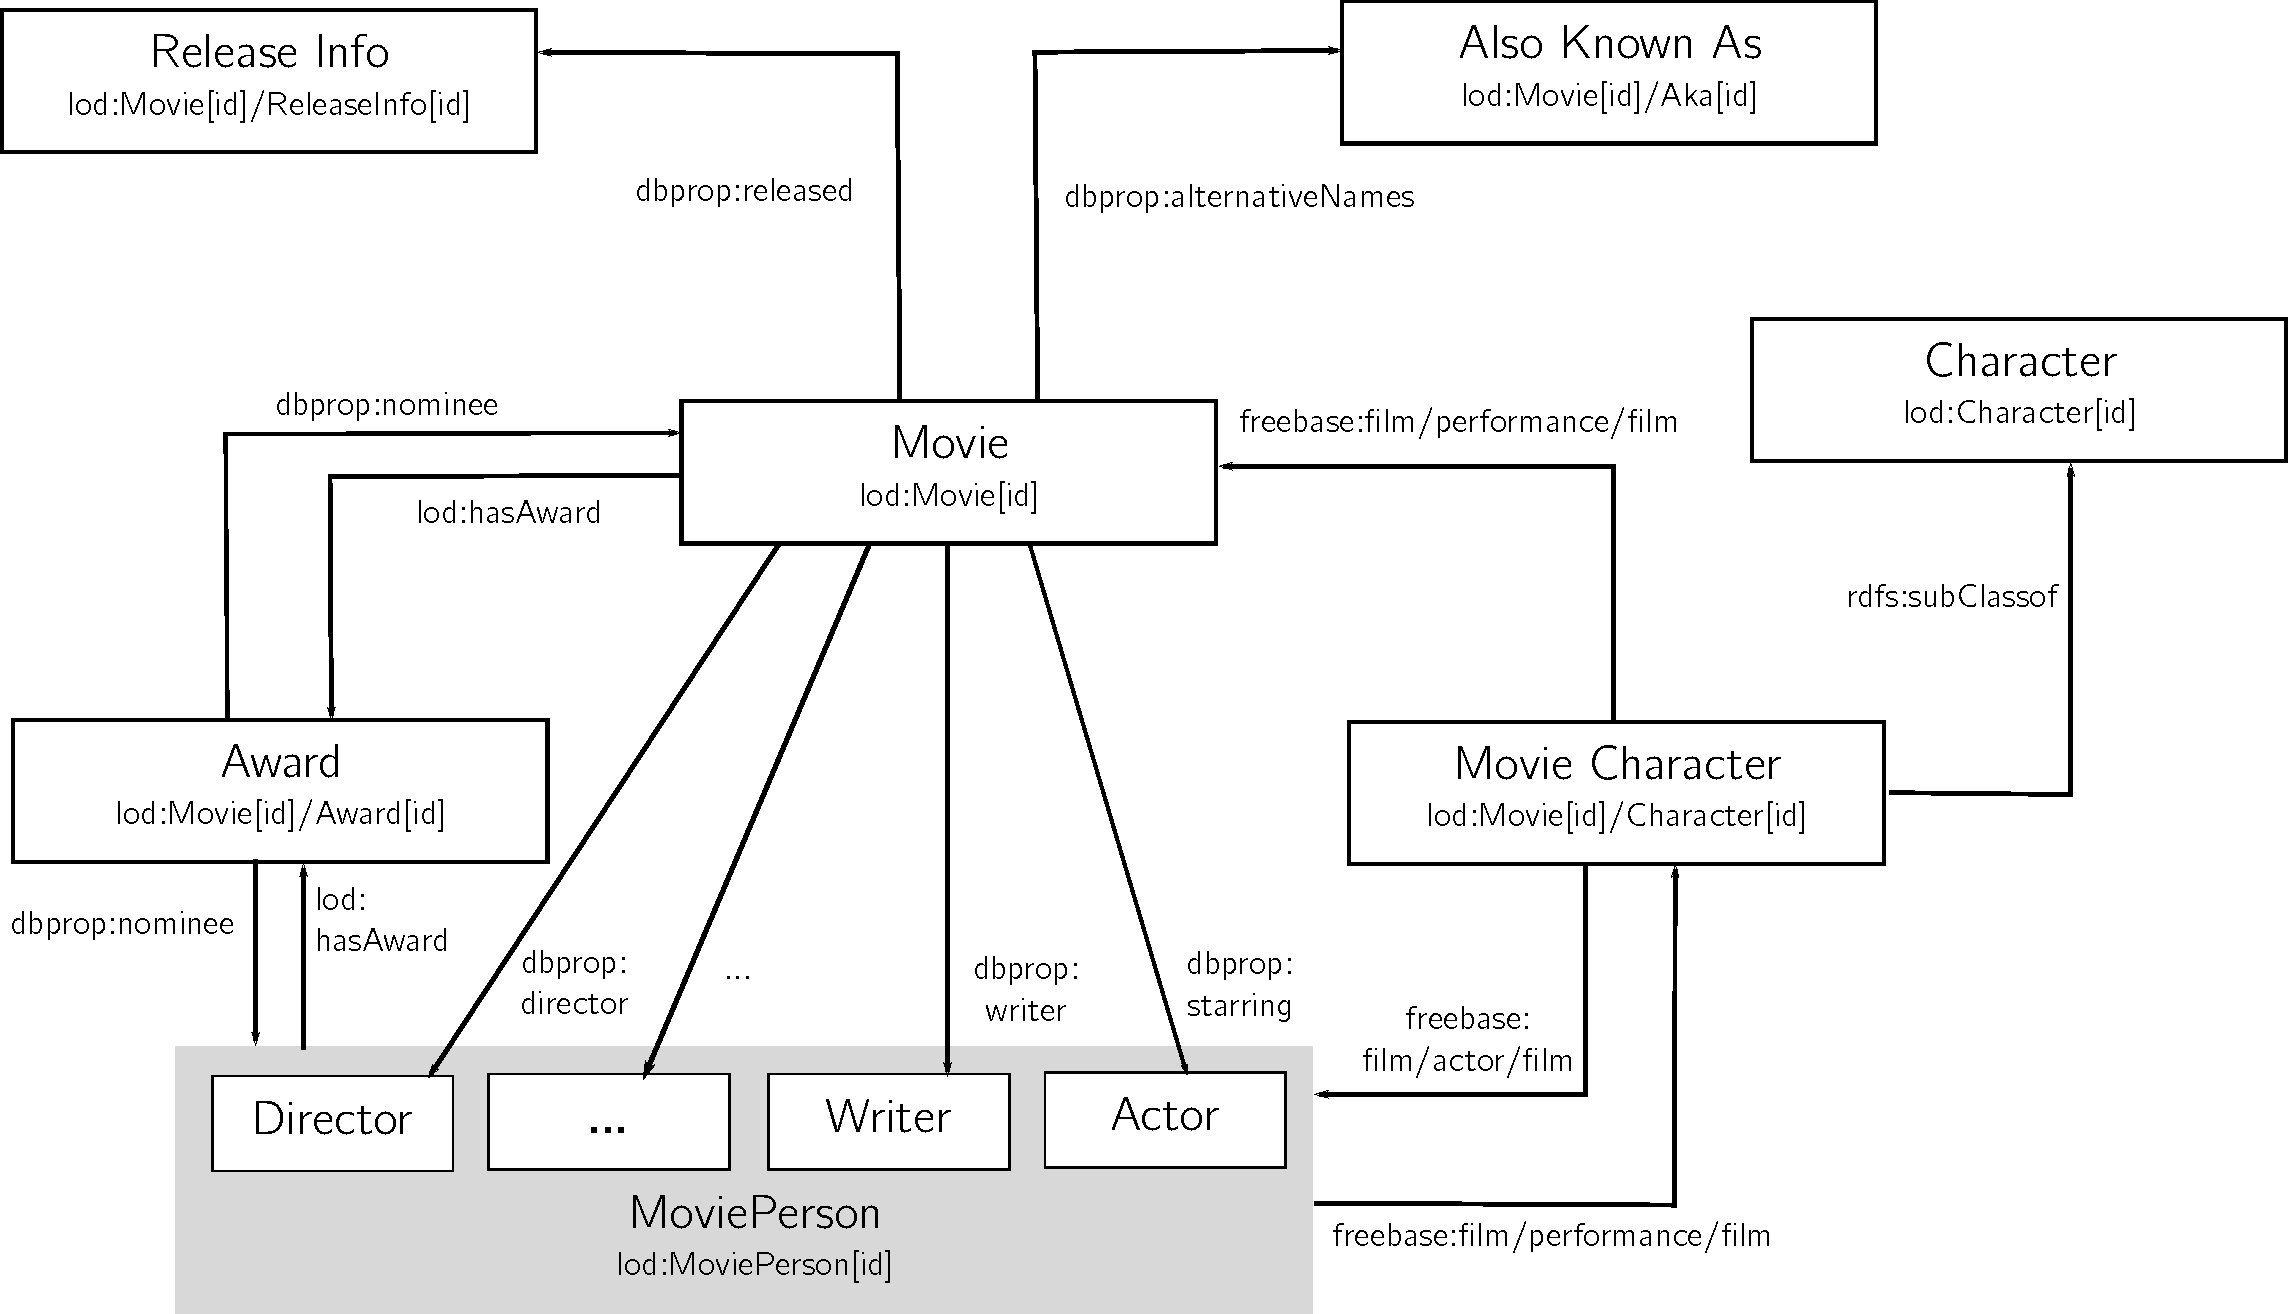
\includegraphics[width=\textwidth]{images/ontology.pdf}
\caption{Ontology}
\label{fig_ontology}
\end{figure}

A \textit{MoviePerson} can have multiple sub-types of \textit{dbpedia-owl:Person}, depending on the jobs the person had in any movies they worked on.
As shown in Figure \ref{fig_ontology} a distinction between e.g. director, writer, producer was made.
For example a person, who is a director in one movie and an actor in another movie, would have the additional classes \textit{dbpedia-owl:Actor} and \textit{dbpedia-owl:Director}.

A problem, which occured when defining our ontology, was the entity \textit{Character}.
In the first definition, there was just one Character class, which was connected to the corresponding movie and actor.
Also the actor had a connection to the character.
The URL of the character was build out of the character name.

Thus, a role which exists in multiple movies (e.g. "cleaning lady") would be one resource connected to each actor who had ever portrayed this role.
The role had also a list of movies, which it occures in.
That way, one could not say, which actors played the role in a certain movie.
One such case is an actor who played a certain role in an old movie but also appears in the movie's newer remake.
In the remake, they might play a different role while another actor plays their original role.
An example for this is the movie "Starsky \& Hutch" (2004), which is a remake of the (1970s) television series with the same name.
In the movie, both actors which originally portrayed Starsky and Hutch get a cameo appearance alongside the new cast for their old roles.

With the old approach, the system could not know who played the Starsky role in the remake, because all actors, who ever played the role, are listed.

Therefore, an additional class of MovieCharacter was introduced in the final ontology.
This resource is only connected to one movie and all actors, who played that role in the movie.
The URL of the MovieCharacter is build from the unique identifier of the movie and the character.
The MovieCharacter is a subclass of \textit{Character}, which describes the general role.
This means, that the unique identifier of the \textit{MovieCharacter} in the "Starsky \& Hutch" example is "Starksy/Starsky\&Hutch1970" and identifier of \textit{Character} is "Starksy".

%TODO ??More detailed description of diagram??
%TODO ??How many total different entity types, relation types, property types??